\section{CAN bus}
\label{sec:Canbus}

Communication between the genset controller and the genset is done via Controller Area Network (CAN) bus. The controller developed in section() which handles the genset frequency, is effectively changing the fuel quantity to the diesel engine. Due to this the communication has to be between the designed controller and the internal engine control.

The CAN bus communication is a type of field bus original designed for use in vehicles and commonly used for control purposed between motors and motor controller. Comparing CAN bus to the open system interconnection (OSI) model the CAN bus consists of three layers. The physical, the data link and the application layer. The lower layers as the physical and data link layers are described in the ISO 11898 standard \cite{CAN_whitepaper_NI}. 

For the physical layer there are generally three different options, a two wire high speed bus that is capable of speeds up to 1Mbit/s when the distance is under 40 meters. Furthermore another two wire option described in ISO 11898-3 is available, this is a low speed fault tolerant version, where the speed is 125kbit/s. The last option is a single wire bus where the speed is limited to 33,3 kbit/s or 83,3 kbit/s in diagnostic mode, this is described in SAE J2411 \cite{CAN_singlewire}.
The logic levels are also specified in these standards. For a two wire CAN bus, a logical 0 corresponds to a high voltage differential between the two communication wires and a logical 1 corresponds to a low voltage differential between the communication wires. This is shown on \figref{fig:CAN_voltage}. 

\begin{figure}[H]
\centering
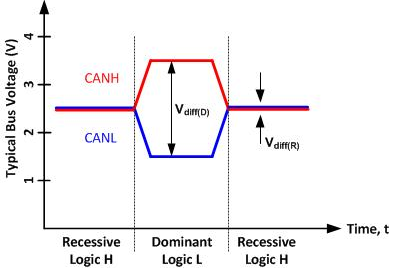
\includegraphics[width=0.75\textwidth]{rapport/billeder/CAN_voltage}
\caption{Voltage levels on a two wire CAN bus \cite{fig_CAN_V_levels}.}
\label{fig:CAN_voltage}
\end{figure}     
%https://e2e.ti.com/blogs_/b/industrial_strength/archive/2015/06/04/what-do-can-bus-signals-look-like
For a single wire CAN bus according to SAE J2411 the recessive and dominant logical values will behave the same, but the voltage differential will be according to ground. 

Concerning the CAN data link layer this can be divided into classical CAN and a new version with flexible data rate called CAN FD, both are described in ISO 11898-1. 
The data link layer will be described for classical CAN, however CAN FD uses the same structure and is therefor backwards compatible if a classical CAN frame is received.

The layout of frames on the CAN bus follow the structure of \figref{fig:CAN_frame}.

\begin{figure}[H]
\centering
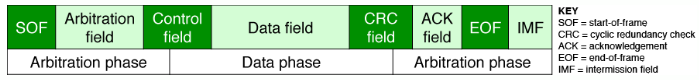
\includegraphics[width=0.75\textwidth]{rapport/billeder/CAN_frame}
\caption{Showing the layout of a CAN bus data frame \cite{fig_CAN_frame}.}
\label{fig:CAN_frame}
\end{figure}

On \figref{fig:CAN_frame} a general CAN bus frame is showed, where SOF is the start-of-frame field. The arbitration field contains an ID of either 11 or 29 bytes and determines the priority where a lower ID yields a higher priority. The control field contains informations about data length and type. The data field contains the actual data which for classical CAN is up to 8 bits and for CAN FD up to 64 bytes. After the data field a 15 bit cyclic redundancy check (CRC) field is present. This is followed by an acknowledgment (ACK) field where nodes that received the message will send an ACK and the transmitting node will listen and either retransmit the data if no ACK is present or end the frame if an ACK is received. This is the general frame structure for CAN bus.   


Depending on the settings of the frame four different message types are available on the CAN bus. 
The frame shown on \figref{fig:CAN_frame} is an example of a data frame, which purpose is to transmit recorded data over the bus. Another frame type is a remote frame which has no data and a specific bit set in the control field to specify it is a remote frame. The purpose of this frame is to request a data frame form other nodes. The last two message types are error frames and overload frames, where the error frame consists of a six bit error flag and an eight bit error delimiter. The structure of the overload frame is similar.  

The CAN bus is structured without a master, instead all nodes are broadcasting to every one else. This implies that transmitting data to a specific node is impossible, as everyone is listening and the message is transmitted on the entire bus. In order for a node to transmit on the bus, it checks if the bus is free and if that is the case it transmits. This structure can results in message collisions as two nodes both waiting for the bus to become free will start transmitting at the same time. In order to solve this and select which note should transmit, the arbitration field is used, where the node with the lowest ID wins. This behavior is due to the dominant property of logital 0 which naturally favors lower arbitration ID's, this can be seen on \figref{fig:CAN_arbitration}.  

\begin{figure}[H]
\centering
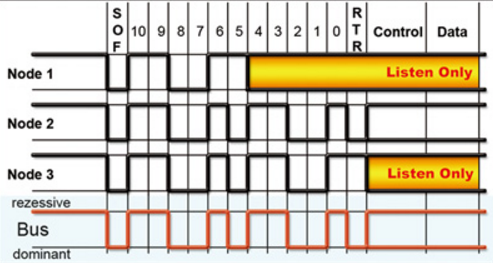
\includegraphics[width=0.75\textwidth]{rapport/billeder/CAN_arbitration}
\caption{Showing arbitration behavior on a CAN bus \cite{fig_CAN_arbitation}.}
\label{fig:CAN_arbitration}
\end{figure}
%http://www.icpdas.com/root/product/solutions/industrial_communication/fieldbus/can_bus/can_intro.html

A communication example of three nodes on a CAN bus network is shown on \figref{fig:CAN_arbitration}. Here the transmitted signals from the nodes is shown in black and the signal on the CAN bus is shown in red. The example shows that when node one tries to transmit a logical 1 as the other nodes transmit a logical 0 node one will lose arbitration as logical 1 is recessive. After this, node one will only listen to the bus and wait until it is not occupied. The example also shows that node 3 looses arbitration at the RTR field, which determines weather the frame is a data or remote frame. A remote frame has RTR set as recessive, therefore data frames are prioritized higher than remote frames in CAN bus and node two wins arbitration.   



%\begin{figure}[H]
%\centering
%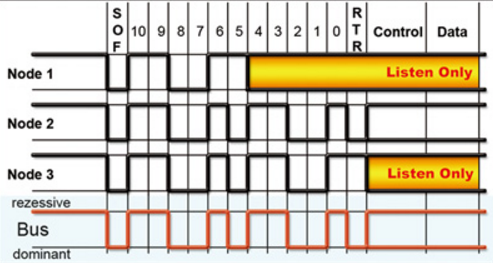
\includegraphics[width=0.75\textwidth]{rapport/billeder/CAN_arbitration}
%\caption{.}
%\label{fig:blok}
%\end{figure}

%1* highspeed can, 2 wires, up to 1Mbit/s  ISO 11898-2
%2* Lowspeed can (fault tolerant), 2 wires,  up to 125 kbit/s 11898-3
%3* Single wire can, 33,3 kbit/s or 83,3 kbit/s in high-speed diagnistics mode, 

%1*
%http://digital.ni.com/public.nsf/allkb/84210794086E9C0886256C1C006BE6AE



%2*
%http://digital.ni.com/public.nsf/allkb/84210794086E9C0886256C1C006BE6AE



%3*
%SAE J2411 (https://www.can-cia.org/can-knowledge/can/sae-j2411-single-wire/)


%alle
%https://www.kvaser.com/can-protocol-tutorial/
%http://www.ni.com/white-paper/2732/en/

%CAN FD
%https://www.kvaser.com/about-can/can-fd/